\section{Resultados y discusión}

Esta sección integra las reconstrucciones y métricas generadas con la configuración descrita. La interpretación se limita a los filtros evaluados, al fantoma usado y a la realización de ruido considerada.

\subsection*{Reconstrucciones sin ruido}

La Figura~\ref{fig:chapter3-recon-noiseless} muestra las reconstrucciones obtenidas a partir del sinograma sin ruido. Visualmente, la rampa recupera la estructura principal del fantoma y obtiene el menor error relativo, mientras que los filtros E y D producen resultados cercanos entre sí según las métricas de la Tabla~\ref{tab:chapter3-metrics}.

\begin{figure}[htbp]
    \centering
    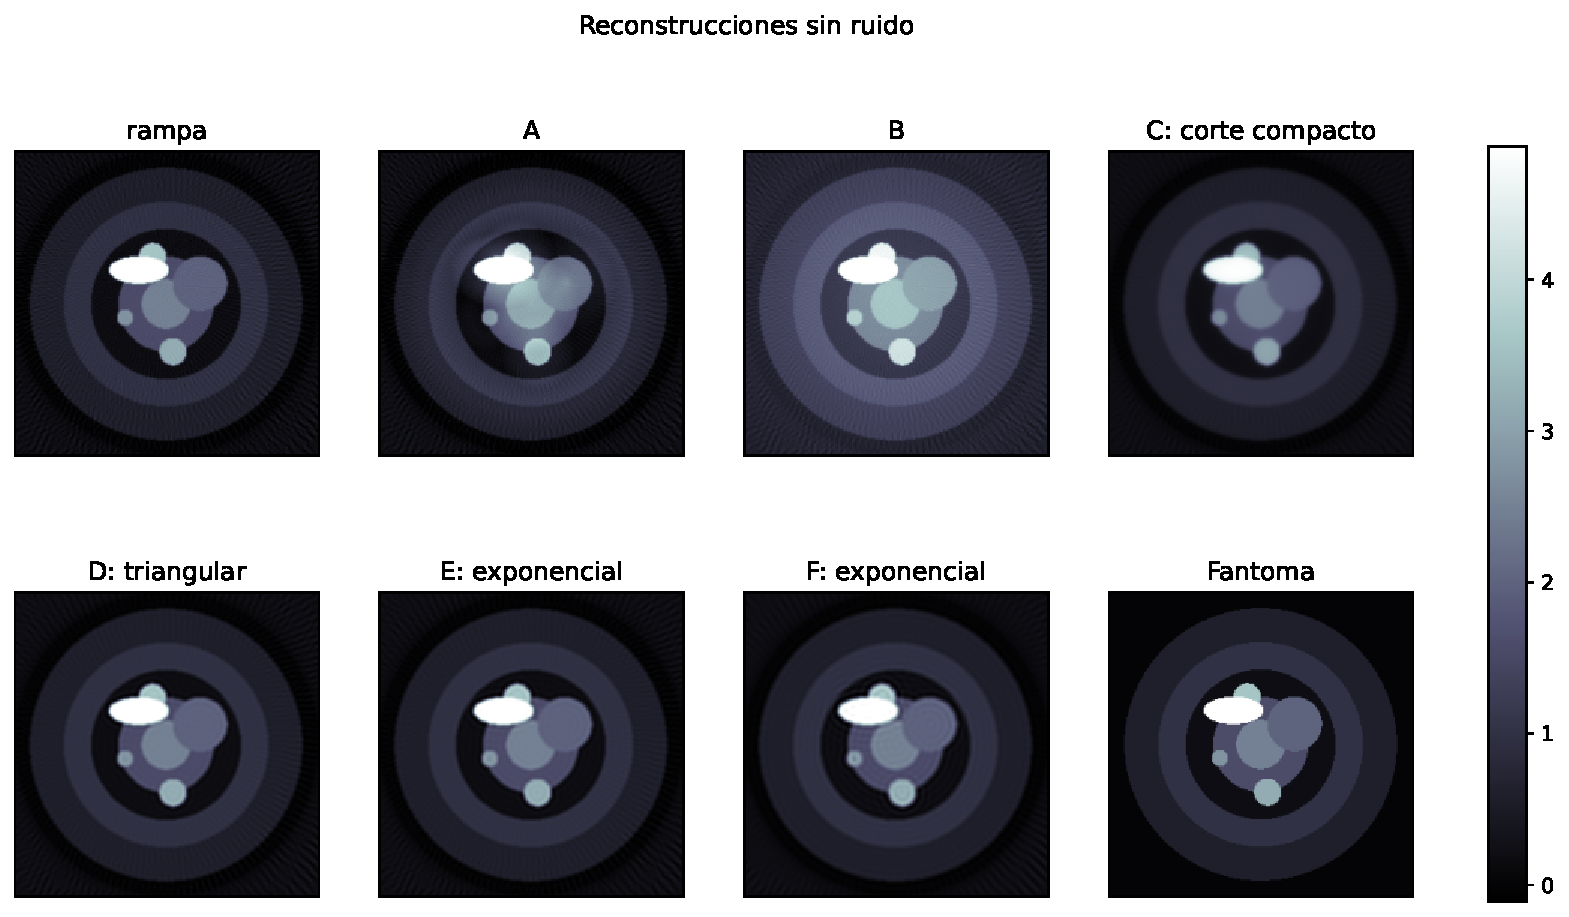
\includegraphics[width=0.96\textwidth]{Figures/Chapter3/reconstructions_noiseless.pdf}
    \caption{Reconstrucciones obtenidas sin ruido para la rampa y los filtros A--F. El último panel muestra el fantoma de referencia bajo la misma escala de color usada para las reconstrucciones, lo que permite comparar amplitud y estructura visual.}
    \label{fig:chapter3-recon-noiseless}
\end{figure}

En términos de error relativo, el menor valor sin ruido corresponde a la rampa, con $0.097892$. Le siguen E, con $0.112767$, y D, con $0.113110$; la diferencia entre estos dos filtros es pequeña en esta configuración. F obtiene $0.127115$ y C alcanza $0.143042$, mientras que A y B presentan errores mayores, $0.253226$ y $0.687715$, respectivamente.

\subsection*{Reconstrucciones con ruido}

La Figura~\ref{fig:chapter3-recon-noisy} muestra las reconstrucciones obtenidas a partir del sinograma perturbado con ruido gaussiano. Bajo la realización de ruido considerada, los filtros que atenúan altas frecuencias reducen de forma marcada la amplificación del ruido respecto de la rampa.

\begin{figure}[htbp]
    \centering
    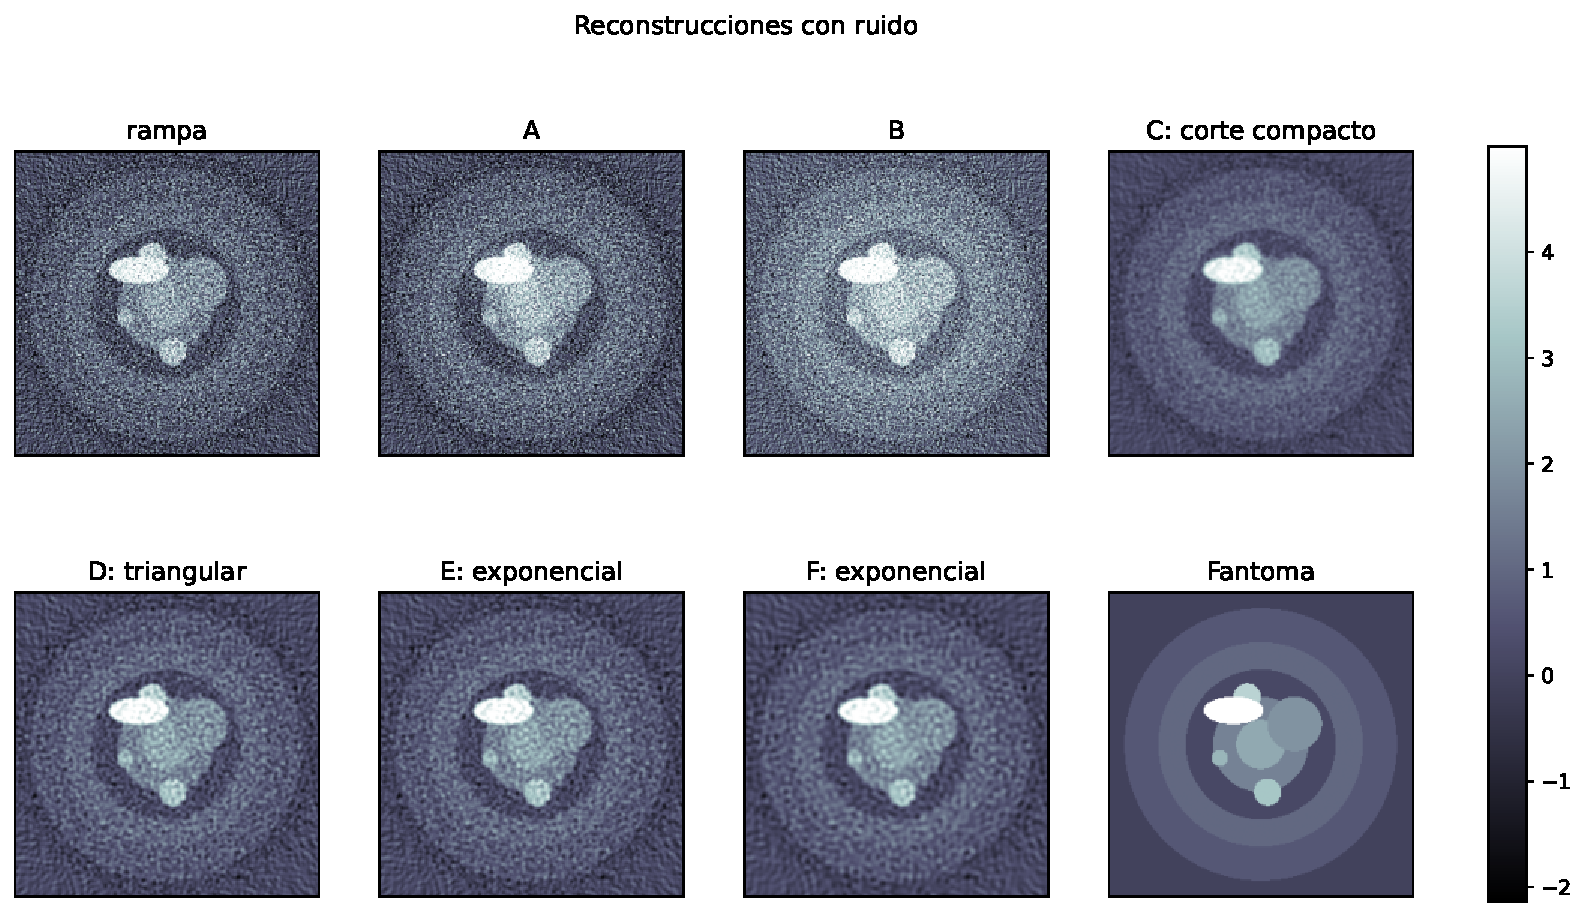
\includegraphics[width=0.96\textwidth]{Figures/Chapter3/reconstructions_noisy.pdf}
    \caption{Reconstrucciones obtenidas a partir de un único sinograma ruidoso, común a todos los filtros. Las diferencias visuales reflejan el compromiso entre preservación de detalle y atenuación de altas frecuencias bajo la realización de ruido considerada.}
    \label{fig:chapter3-recon-noisy}
\end{figure}

Entre los filtros evaluados, C obtiene el menor error relativo con ruido, $0.266386$, seguido por F con $0.318981$. Los filtros E y D quedan en un rango intermedio, con $0.383664$ y $0.390949$, respectivamente. La rampa y A presentan errores relativos mayores, $1.134227$ y $1.157932$, consistentes con una mayor amplificación de altas frecuencias. El filtro B alcanza $1.323399$; su comportamiento desfavorable es consistente con su respuesta no nula en frecuencia cero y su mayor peso de bajas frecuencias, aunque este experimento no constituye una demostración causal completa.

\subsection*{Métricas cuantitativas}

La Tabla~\ref{tab:chapter3-metrics} resume RMSE, error relativo y razón de medias. RMSE y error relativo son las métricas principales. La razón de medias se incluye únicamente como diagnóstico de amplitud y no se usa para reescalar ni para seleccionar filtros.

\begin{table}[htbp]
    \centering
    \caption{Métricas de reconstrucción calculadas sobre los índices $\mathcal I_R=\{(i,j):x_i^2+y_j^2\le R^2\}$. RMSE y error relativo en norma $\ell^2$ son las métricas principales; la razón de medias se reporta únicamente como diagnóstico de amplitud.}
    \label{tab:chapter3-metrics}
    \small
    \begin{tabular}{llrrr}
\toprule
Caso & Filtro & RMSE & Error relativo $\ell^2$ & Razón media \\
\midrule
sin ruido & rampa & 0.125294 & 0.097892 & 0.976683 \\
sin ruido & A & 0.324107 & 0.253226 & 1.181567 \\
sin ruido & B & 0.880214 & 0.687715 & 1.906510 \\
sin ruido & C: corte compacto & 0.183081 & 0.143042 & 0.963424 \\
sin ruido & D: triangular & 0.144770 & 0.113110 & 0.975620 \\
sin ruido & E: exponencial & 0.144332 & 0.112767 & 0.975596 \\
sin ruido & F: exponencial & 0.162695 & 0.127115 & 0.975090 \\
con ruido & rampa & 1.451709 & 1.134227 & 0.978050 \\
con ruido & A & 1.482050 & 1.157932 & 1.183776 \\
con ruido & B & 1.693833 & 1.323399 & 1.908387 \\
con ruido & C: corte compacto & 0.340951 & 0.266386 & 0.964867 \\
con ruido & D: triangular & 0.500380 & 0.390949 & 0.977034 \\
con ruido & E: exponencial & 0.491055 & 0.383664 & 0.977022 \\
con ruido & F: exponencial & 0.408268 & 0.318981 & 0.976554 \\
\bottomrule
\end{tabular}

\end{table}

Los resultados ilustran el compromiso entre resolución y estabilidad: sin ruido, las respuestas próximas a la rampa conservan mejor los detalles; con ruido, atenuar altas frecuencias reduce el error a costa de suavizado. El desempeño de C se limita a esta configuración y realización de ruido, sin implicar superioridad universal.
